\chapter{Framework results}
The framework is tested using the reference design of a FIR-filter, described in \cref{subsec:refdesfir}. The source code of the filter, written in C, is listed in \cref{subsec:cfircode} in the appendix. The implemented FIR-filter has a 32-bit input, 16 taps and 64-bit output. The filter-coefficients are for simplicity defined to be the integers 1-16. By running this design through the framework, we will get multiple results. These results will be compared towards each other, but also towards the same FIR-filter implemented in Verilog directly. The source code of the Verilog implementation is listed in \cref{subsec:verilogfircode} in the appendix.

\section{\label{sec:firstrun}First test-run}
The first test-run were performed with 6 randomized constraints input to LegUp. Each of the constraints could take values 1 and 0, giving a total of $2^6=64$ combinations. The randomized constraints and the pattern of how the values are set is shown in \cref{tab:randomconstraint}.

\begin{table}
\tiny
    \begin{center}
    \begin{tabular}{l|cccccc}
     & & & \textbf{MB} & \textbf{ENABLE} & \textbf{DUAL} & \\
          &
          \textbf{SDC NO} & 
          \textbf{PIPELINE} & 
          \textbf{MINIMIZE} & 
          \textbf{PATTERN} & 
          \textbf{PORT} &
          \textbf{CASE} \\
        \textbf{Constraint}
           & \textbf{CHAINING}
           & \textbf{ALL}
           & \textbf{HW}
           & \textbf{SHARING}
           & \textbf{BINDING}
           & \textbf{FSM}
    \\ \midrule
    & 0 & 0 & 0 & 0 & 0 & 1 \\
    & 0 & 0 & 0 & 0 & 1 & 0 \\
    & 0 & 0 & 0 & 0 & 1 & 1 \\
    \textbf{Value} & \vdots & \vdots & \vdots & \vdots & \vdots & \vdots \\
    & &  &  &  &  &  \\
    & 1 & 1 & 1 & 1 & 1 & 0 \\
    & 1 & 1 & 1 & 1 & 1 & 1
    \\ \bottomrule
    \end{tabular}
    \caption{\label{tab:randomconstraint}Constraints and values for first run}
    \end{center}
\end{table}

This framework run only included HLS, simulation, and synthesis, as the layout and power estimation tools were not yet incorporated into the framework flow. Synthesis is run using a 32MHz clock and a 180nm cell library. A simple testbench generated by LegUp, with testcases similar to the ones listed in \cref{lst:tbcases}, were used for this run. 

The presented results are gathered from the synthesis reports. The generated Verilog for many of the constraint files synthesize into the exact same area consumption and. This indicates that some of the combinations are redundant. The results are shown in \cref{tab:hlsrun1dataresults}. As there are only 8 different results, only $log_2(8) = 3$ constraint parameters affect the design, the other will be don't-care constraints. By converting the design number to binary, the first row of the result table is shown in \cref{tab:dectobinconstraints}, a pattern can be seen and that the parameters \textit{PIPELINE\_ALL}, \textit{ENABLE\_PATTERN\_SHARING} and \textit{DUAL\_PORT\_BINDING} are don't care for the this design.

The area results are given in cell units, dynamic and total power are given in milliWatts (mW), and leakage power is given in nanoWatts (nW).


\begin{table}[hbtp]
    \centering
    \begin{tabular}{ccccc}
    & & \multicolumn{3}{c}{\textbf{Power}} \\
    \cline{3-5}
    \textbf{Design \#} & \textbf{Area} & \textbf{Dynamic} & \textbf{Leakage} & \textbf{Total} \\
    \toprule
    Verilog & 175517.771501 & 2.9522 & 13.2559 & 2.9522 \\
    9,11,13,15,25,27,29,31 & 542636.067533 & 1.1933 & 445.5482 & 1.1937 \\
    8,10,12,14,24,26,28,30 & 543715.713936 & 1.1909 & 442.7919 & 1.1913 \\
    41,43,45,47,57,59,61,63 & 570759.857112 & 1.3097 & 474.8710 & 1.3102 \\
    1,3,5,7,17,19,21,23 & 571069.521032 & 1.2792 & 467.3262 & 1.2797 \\
    0,2,4,6,16,18,20,22 & 574368.902419 & 1.2745 & 467.3031 & 1.2750 \\
    40,42,44,46,56,58,60,62 & 574468.505099 & 1.3100 & 475.3570 & 1.3105 \\
    33,35,37,39,49,51,53,55 & 598731.305489 & 1.3951 & 498.4164 & 1.3956 \\
    32,34,36,38,48,50,52,54 & 599552.442242 & 1.3949 & 500.0916 & 1.3954 \\
    \bottomrule
    \end{tabular}
    \caption{Results from first framework run}
    \label{tab:hlsrun1dataresults}
\end{table}

\begin{table}[hbtp]
    \centering
    \begin{tabular}{cccc}
    \textbf{Decimal} & \textbf{Binary}\\
    \toprule
    9 & 001001 \\
    11 & 001011 \\
    13 & 001101 \\
    15 & 001111 \\
    25 & 011001 \\
    27 & 011011 \\
    29 & 011101 \\
    31 & 011111 \\
    \bottomrule
    \end{tabular}
    \caption{Decimal to binary conversion shows the pattern in the constraints}
    \label{tab:dectobinconstraints}
\end{table}

\begin{figure}[hbpt]
\centering
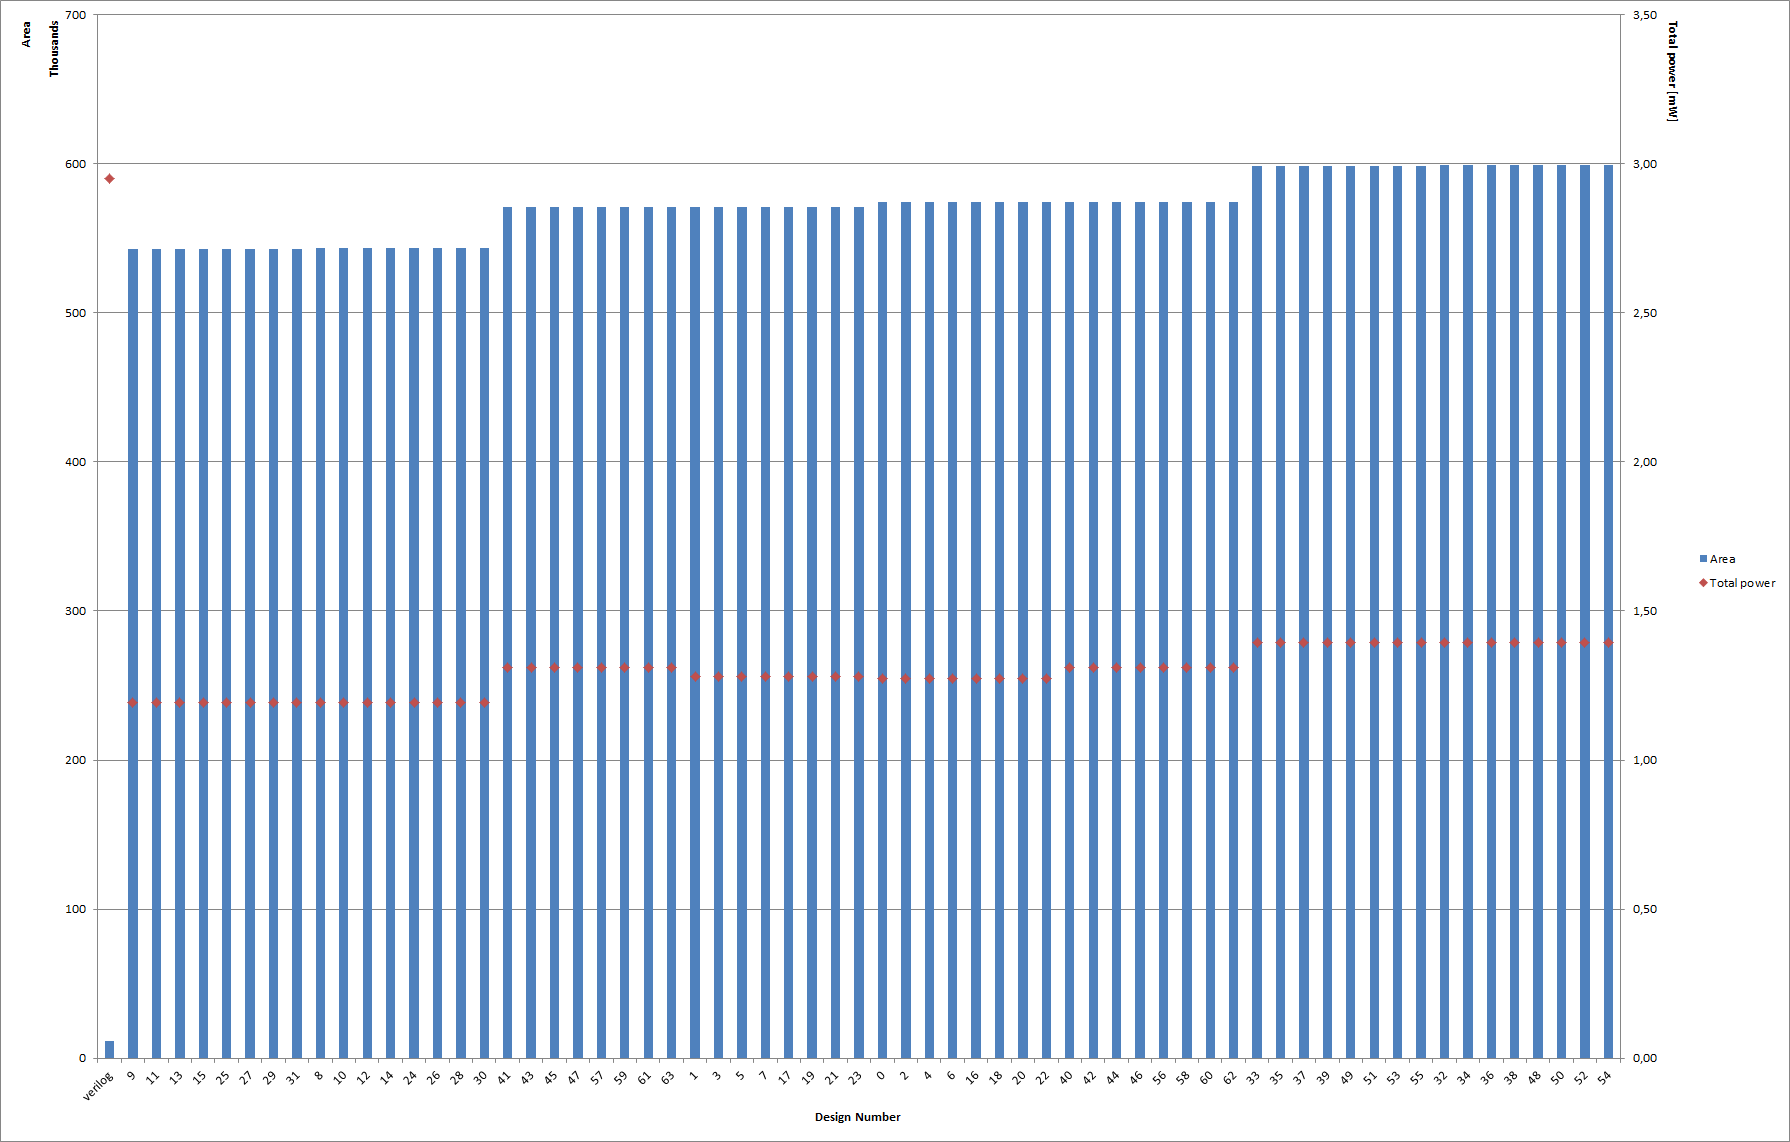
\includegraphics[width=\textwidth]{../figs/resultGraph.png}
\caption{\label{fig:resultgraphhlsrun1}Graph of results from first HLS run}
\end{figure}
The best result with regards to area is the ones with the parameters \textit{SDC\_NO\_CHAINING} set to 0, \textit{MB\_MINIMIZE\_HW} set to 1 and \textit{CASE\_FSM} set to 1. The best result with regards to total power consumption is the same as for area, just with \textit{CASE\_FSM} set to 0.

The results are visualized in \cref{fig:resultgraphhlsrun1}. It is clear from the graph that the concept is working as expected and that we get different result for different constraints. In \cref{fig:resultcomparisonhlsrun1}, the best area-result from the framework is compared towards the results from the same design written in Verilog directly. It is clear from the graph that the design written directly in Verilog is way better in terms of area consumption, it does not make sense that the estimated power consumption of the design in Verilog is much higher than the HLS-generated design.

\begin{figure}[hbpt]
\centering
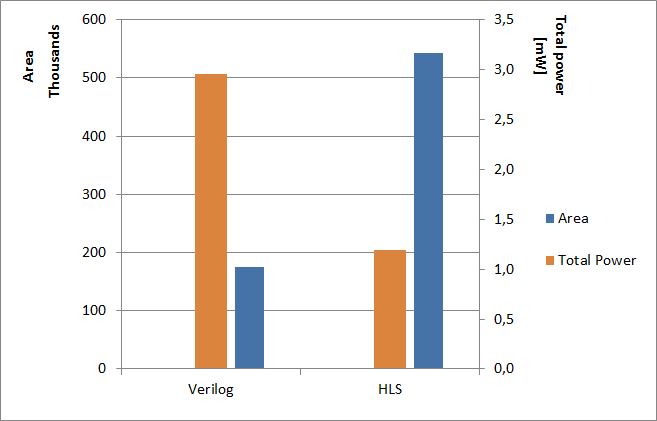
\includegraphics[width=0.75\textwidth]{../figs/resultComparison1.png}
\caption{\label{fig:resultcomparisonhlsrun1}Graph comparing framework generated design towards same design written in Verilog}
\end{figure}

\subsection{Handling unexpected results}
It seems strange that the area consumption of the design written in Verilog is just 32.3\% of the best result from LegUp, while the power consumption of the design written in Verilog is 247.4\% of the best result from LegUp. Typically a larger design will consume more power, as each of the components has leakage and static operation consumption. Notice that this results were obtained using a static power estimation tool, the amount of switching in gates and registers has not been taken into account. However, this unexpected result needed to be investigated further. The following steps were taken to ensure the quality of the results to be acceptable:

\begin{itemize}
    \item Check generated reports for misinterpreted data
    \item Look at schematic view of synthesized design to find errors
    \item Run HLS and synthesis once more to see if results deviates
\end{itemize}

None of the two first steps showed any errors. The designs are however too large to make any sense of the schematics, and due to to the limitation in setting signal sizes in the C-code, the HLS-generated Verilog designs scale down very poorly. The third step were performed on the same design, but with the clock relaxed from 32MHz to 16MHz. Changing the clock should not affect the design that much, but the synthesis will try to optimize the circuit to use the least amount of area, but still meet timing requirements. This time, only the constraints that had an impact on the design were included, generating 8 different designs. The result of the second run is shown in \cref{tab:resultgraphframeworkrun2} and in \cref{fig:resultgraphframeworkrun2}.
\begin{table}[hbtp]
    \centering
    \begin{tabular}{ccccc}
    & & \multicolumn{3}{c}{\textbf{Power}} \\
    \cline{3-5}
    \textbf{Design \#} & \textbf{Area} & \textbf{Dynamic} & \textbf{Leakage} & \textbf{Total} \\
    \toprule
    Verilog & 175531.077145 & 1.0961 & 291.4545 & 1.0964 \\
    3 & 736221.630958 & 3.0417 & 600.7903 & 3.0423 \\
    2 & 738362.360388 & 3.0424 & 603.0359 & 3.0430 \\
    0 & 766630.553023 & 3.1736 & 627.3008 & 3.1742 \\
    1 & 783120.518084 & 3.2230 & 641.3857 & 3.2236 \\
    7 & 796905.744222 & 3.0702 & 634.3779 & 3.0708 \\
    6 & 798087.595262 & 3.0693 & 635.5286 & 3.0699 \\
    4 & 830305.921961 & 3.2036 & 660.1381 & 3.2043 \\
    5 & 853504.409992 & 3.2898 & 681.0897 & 3.2905 \\

    \bottomrule
    \end{tabular}
    \caption{Results from second framework run.}
    \label{tab:resultgraphframeworkrun2}
\end{table}

\begin{figure}[hbpt]
\centering
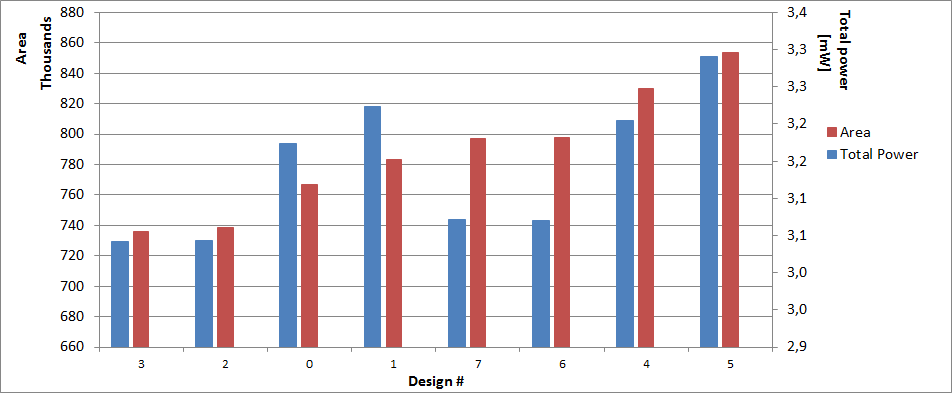
\includegraphics[width=\textwidth]{../figs/resultGraph2.png}
\caption{\label{fig:resultgraphframeworkrun2}Graph of results from second framework run}
\end{figure}

These results are a better match with our expectations. Both area and power has increased a bit for all HLS-generated designs. The reason for this is not known, but there could have been a bug in the design or a setting in the first run that generated odd results. When comparing the best HLS result towards the design written in Verilog, as shown in \cref{fig:resultcomparisonhlsrun2}, we see that the Verilog design has both lower area and power consumption, which is what would be expected.

\begin{figure}[hbpt]
\centering
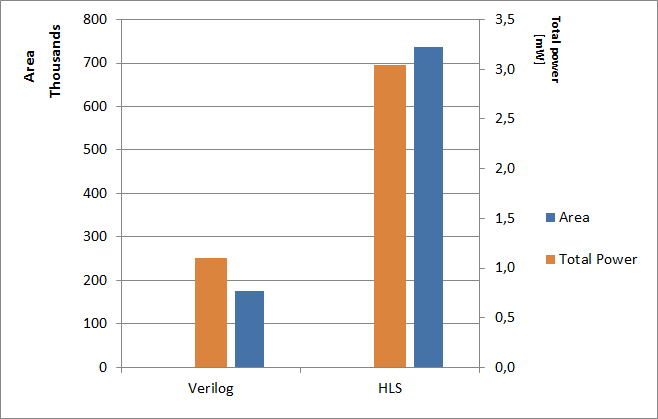
\includegraphics[width=0.75\textwidth]{../figs/resultComparison2.png}
\caption{\label{fig:resultcomparisonhlsrun2}Graph comparing framework generated design from second run towards same design written in Verilog}
\end{figure}

\section{Full tool-flow framework run}
The full tool-flow were incorporated into the framework, to see if more accurate power estimates shows a different result. With the full tool-flow, the area reports is gathered from layout instead of synthesis and the power estimates is gathered from power analysis. The full tool-flow is run using the same design as in \cref{sec:firstrun}, with only the three constraints that affected the output, again a total of 8 designs. Since the full tool-flow uses switching data from the simulation to perform power analysis, the testbench used had to be changed to get more switching values. The new testbench applies 1000 random inputs to the input \textit{inData} and waits for the flag \textit{iterationFinished} to be set before applying a new input. The full source code of this testbench is listed in \cref{subsec:firfiltertb}. The testbench for the design written in Verilog is almost exacly the same, just adapted to the correct signal names and instead of waiting for a flag, \textit{inData} is assigned a new value each 17 clock cycles. The area results are shown in \cref{tab:resultgraphareaframeworkrun2} and the power estimates are shown in \cref{tab:resultgraphpowerframeworkrun2}.

\begin{table}[hbtp]
    \centering
    \begin{tabular}{cccc}
    & \multicolumn{3}{c}{\textbf{Area}} \\
    \cline{2-4}
    \textbf{Design \#} & \textbf{Combinational} & \textbf{Non-combinational} & \textbf{Total} \\
    \toprule
    Verilog & 72818.22296 & 44647.6792 & 117465.9022 \\
    3 & 130953.7155 & 201114.5108 & 332068.2263 \\
    2 & 131389.4738 & 201114.5108 & 332503.9847 \\
    0 & 136182.8164 & 210973.9603 & 347156.7766 \\
    1 & 139276.3681 & 213895.2786 & 353171.6467 \\
    7 & 136262.6501 & 220468.2449 & 356730.8950 \\
    6 & 137237.2853 & 220468.2449 & 357705.5302 \\
    4 & 141315.4518 & 230327.6944 & 371643.1462 \\
    5 & 146770.7475 & 236170.3311 & 382941.0786 \\
    \bottomrule
    \end{tabular}
    \caption{Area results from framework run with full tool-flow}
    \label{tab:resultgraphareaframeworkrun2}
\end{table}

\begin{table}[hbtp]
    \centering
    \begin{tabular}{ccccc}
    & \multicolumn{4}{c}{\textbf{Power}} \\
    \cline{2-5}
    \textbf{Design \#} & \textbf{Net switching} & \textbf{Internal} & \textbf{Leakage} & \textbf{Total} \\
    \toprule
    Verilog & 0.365 & 1.760 & 100.340 & 2.125 \\
    2 & 1.214 & 5.157 & 281.820 & 6.371 \\
    3 & 1.236 & 5.270 & 273.940 & 6.507 \\
    6 & 1.184 & 5.484 & 293.960 & 6.669 \\
    0 & 1.273 & 5.518 & 292.400 & 6.792 \\
    1 & 1.279 & 5.517 & 307.760 & 6.797 \\
    7 & 1.255 & 5.567 & 267.960 & 6.822 \\
    4 & 1.238 & 5.696 & 308.180 & 6.934 \\
    5 & 1.269 & 5.771 & 327.280 & 7.041 \\
    \bottomrule
    \end{tabular}
    \caption{Power estimation results from framework run with full tool-flow.}
    \label{tab:resultgraphpowerframeworkrun2}
\end{table}

In \cref{fig:resultgraphframeworkrun3} the final area and power estimation results are visualized together. It is clear from the graphs that the concept works, as we get different results from the designs. These results are considered more accurate, as they use the reports from the chip layout for area, and power estimation using switching activity from simulation. Notice that compared to the results from synthesis, the area is actually cut by half, but the estimated power consumption has nearly doubled. This is because the layout tool can run optimizations on the design, decreasing the area, while the power estimates takes the dynamic switching activity into account, increasing the total power consumption. In \cref{fig:resultgraphpowerframeworkrun2}, the area and power estimates from the framework is compared against the same design written directly in Verilog. Here we see the same trend as shown in the synthesis results above, but the relationship between area and power consumption shows more resemblance.

\begin{figure}[hbpt]
\centering
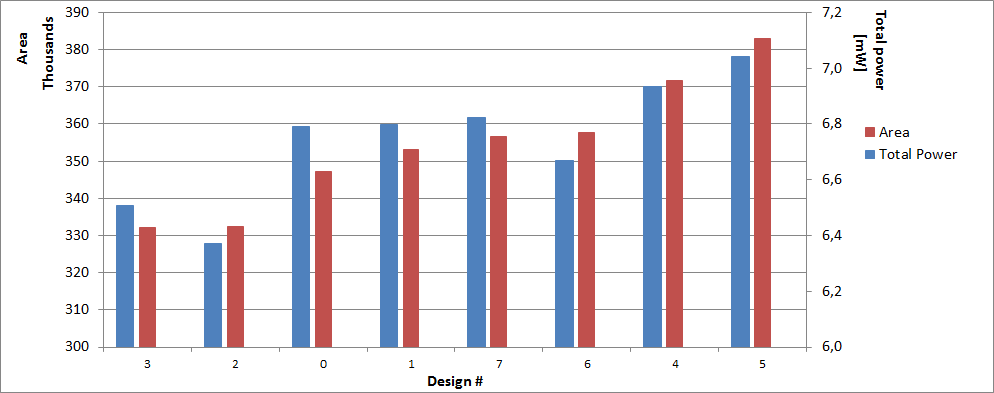
\includegraphics[width=\textwidth]{../figs/resultGraph3.png}
\caption{\label{fig:resultgraphframeworkrun3}Graph of results from framework with full tool-flow}
\end{figure}

\begin{figure}[hbpt]
\centering
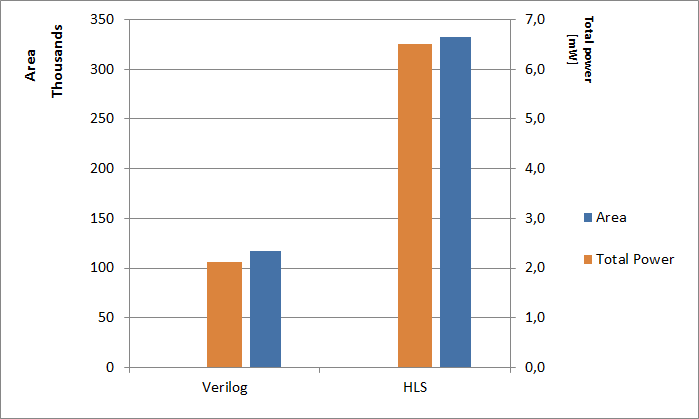
\includegraphics[width=0.75\textwidth]{../figs/resultComparison3.png}
\caption{\label{fig:resultcomparisonhlsrun3}Graph comparing framework generated design from full tool-flow towards same design written in Verilog}
\end{figure}

\cref{fig:resultgraphareaframeworkrun2} and\cref{fig:resultgraphpowerframeworkrun2} shows the distribution of area and power consumption within the designs. In the power graphs, lekage power is not shown as this is negligible compared to the other factors. The trend is the same in all the HLS generated designs, the larger portion of the area is consumed by non-combinational area. In the Verilog designs, the area distribution is inverted. This difference is what is expected from a FSM vs not-FSM design. In the power distribution graph we see that most of the power is consumed internally in the cells both in HLS generated designs and the Verilog design.

\begin{figure}[hbpt]
\centering
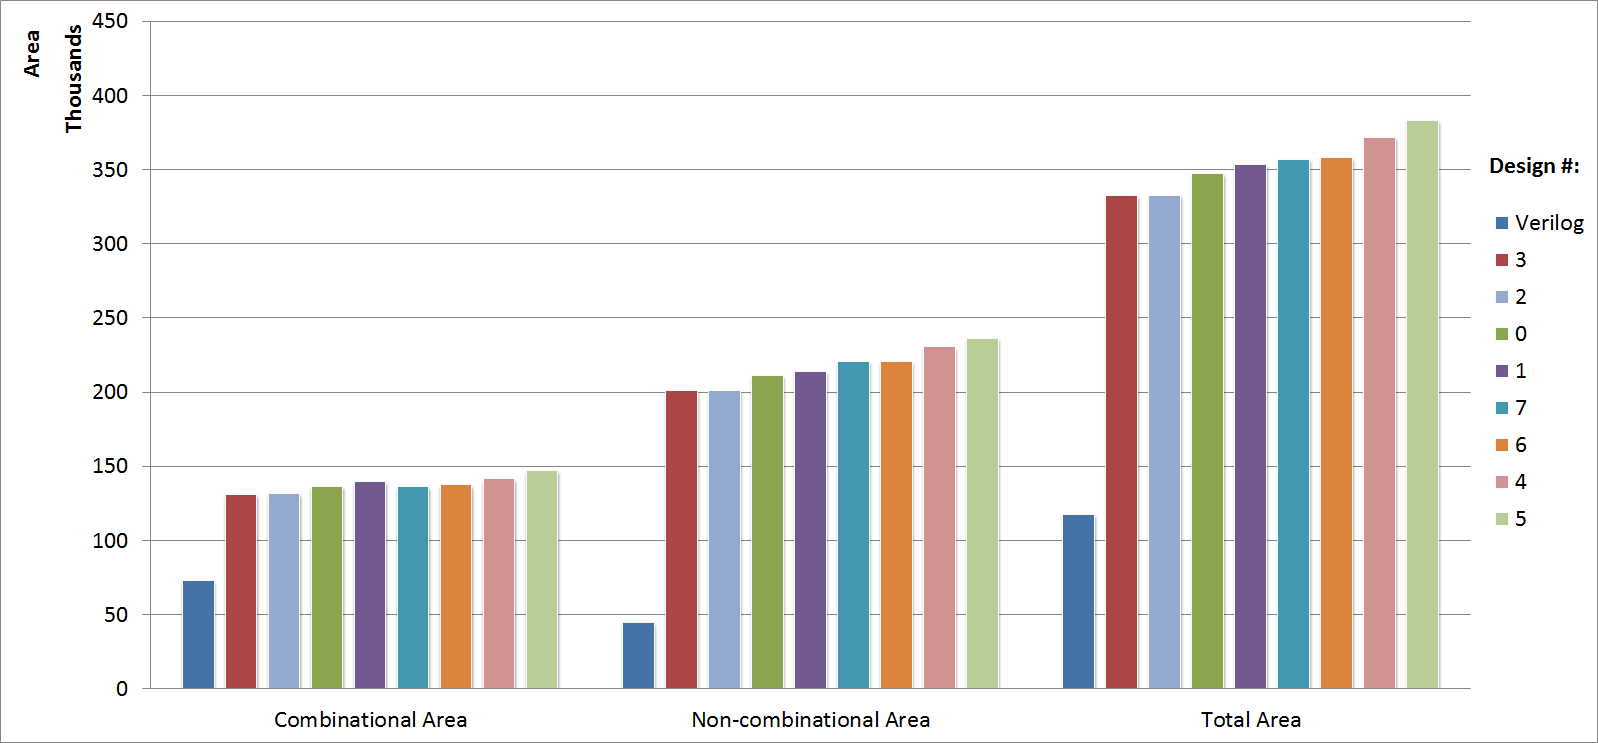
\includegraphics[width=\textwidth]{../figs/resultGraphAreaDistribution.png}
\caption{\label{fig:resultgraphareaframeworkrun2}Graph of area distribution of results from framework with full tool-flow}
\end{figure}

\begin{figure}[hbpt]
\centering
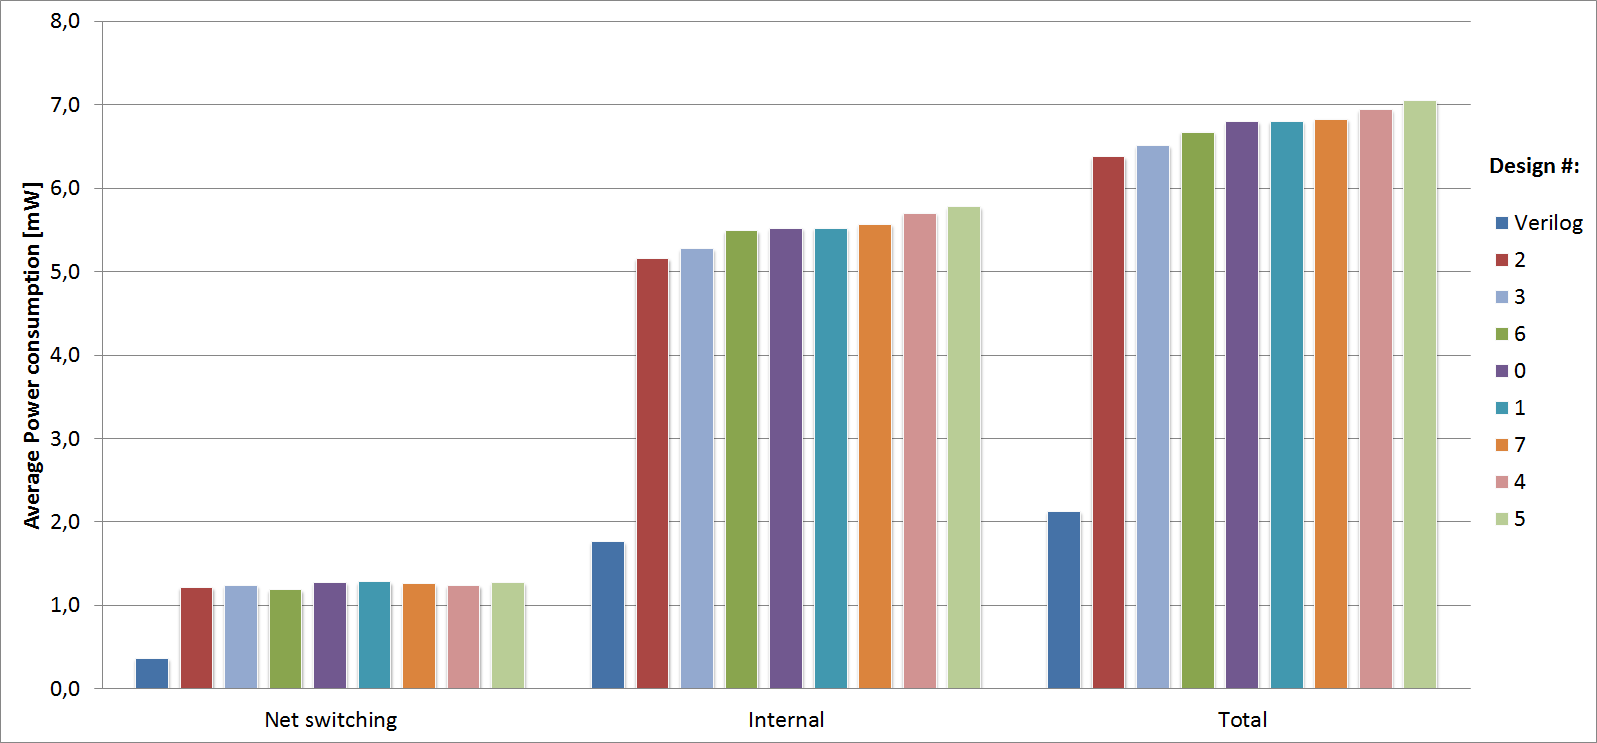
\includegraphics[width=\textwidth]{../figs/resultGraphPowerDistribution.png}
\caption{\label{fig:resultgraphpowerframeworkrun2}Graph of power distribution of results from framework with full tool-flow}
\end{figure}

Another interesting parameter to compare is the number if generated registers. For the implemented design, a minimum of 480 1-bit registers (\verb!INPUTSIZE*(TAPS-1)!) is needed for the shift register, the \textit{sr}-array. The number of registers, gathered from the synthesis reports, is shown in \cref{tab:resultregistercount}. 

\begin{table}[hbtp]
    \centering
    \begin{tabular}{cc}
    \textbf{Design \#} & \textbf{Registers} \\
    \toprule
    Verilog & 480 \\
    0 & 2311 \\
    1 & 2343 \\
    2 & 2203 \\
    3 & 2203 \\
    4 & 2523 \\
    5 & 2587 \\
    6 & 2415 \\
    7 & 2415 \\
    \bottomrule
    \end{tabular}
    \caption{Number of used registers for each design}
    \label{tab:resultregistercount}
\end{table}
\section{Bugs in the generated design}
To avoid the generating of a global memory controller, the flag \textit{NO\_INLINE} had to be set to 0 in the Makefile. This introduces two bugs in the generated Verilog; firstly, the signal generated from the parameter \textit{done} is not sampled after the first time, making the program run forever, secondly the statement \verb!products[0] = inData * 1! is only evaluated on the first iteration of the loop, meaning all outputs from the FIR-filter (except the first one) will have a deviation from the correct result, corresponding to \verb!correctResult - inData + firstInData!. From the generated LLVM IR code it looks like the first bug occurs because the comparison of the input \textit{done} being performed in another state than where it is used as loop exit-condition. In the same state, \textit{inData} is sign-extended, as it is a 32-bit variable being assigned to a 64-bit variable. Both these results are stored to temporary registers for use later, as shown below. From the simulation, it can be seen that this particular state is not visited again when the loop has been entered.
\lstset{language=llvm,style=LLVMstyle}
\begin{lstlisting}
%6 = icmp eq i32 %done, 0
%7 = sext i32 %inData to i64
\end{lstlisting}
These bugs are not critical to this case, as both bugs will be identical to each design. As this results is only supposed to show that the concept works, it is not critical that the generated results are accurate, as long as they are accurate relative to each other.
\section{Path and hold violations}
Some of the designs reports violating path length and hold times in synthesis. For a real circuit this would be a problem. To get rid of these violations, the target clock speed during synthesis could be decreased to something below the maximum frequency of the design. However, the clock speed is most of the time the only thing you cannot change in your design, and design compiler will try to create the circuit that meets timing. If timing is not met, the circuit description should be changed. This means that from our methodology, we will generate many circuits and only the ones that meet timing will be presented as an accepted solution. Ideally, the framework would implement a feedback loop, but for the sake of this proof-of-concept, a long list of solutions are produced and only the best ones are selected.

\section{LegUp specific code optimization}

When going trough the register-count from synthesis, it were noticed that the HLS generated designs implemented both the array \textit{sr} and \textit{products} as RAM modules using registers, while in the design written directly in Verilog, the \textit{sr}-array is the only signal using registers. When looking at the following snippet from the FIR-filter source code, listed in \cref{subsec:cfircode}:
\lstset{language=C,style=CStyle}
\begin{lstlisting}
for (int k = 1; k < TAPS ; k++){
    products[k] = sr[k-1] * (k+1);
}
sum = sum + products[i];
\end{lstlisting}
it can easily be seen that this is functionally equivalent to:
\begin{lstlisting}
sum = sum + (sr[i-1] * (i+1));
\end{lstlisting}
This connection should be made either in the compiler or in LegUp, but it were clearly missed. If we also substitute the code:
\begin{lstlisting}
products[0] = inData * 1;
sum = products[0];
\end{lstlisting}
with:
\begin{lstlisting}
sum = inData * 1;
\end{lstlisting}
the whole \textit{products}-array can be removed. When running this optimized code through the framework, the result is much better than without these optimizations. \cref{tab:resultsframeworkrun3} shows the results from the framework run of design 2, the best design with regards to power consumption from the second framework run.

\begin{table}[hbtp]
    \centering
    \begin{tabular}{lr}
    \multicolumn{2}{c}{\textbf{Synthesis}} \\
    \toprule
    Total Area & 358587.628093 \\
    \hline
    Net Switching Power & 0.1340 mW \\
    Internal Power & 1.3203 mW \\
    Leakage Power & 283.1053 nW \\
    \hline
    Total Power & 1.4546 mW \\
    \hline
    Register count & 899 \\ 
    \bottomrule
    & \\
    \multicolumn{2}{c}{\textbf{Layout}} \\
    \toprule
    Combinational Area & 72482.256207 \\
    Non-combinational Area & 82070.787659 \\
    \hline
    Total Area & 154553.043866 \\
    \bottomrule
    & \\
    \multicolumn{2}{c}{\textbf{Power analysis}} \\
    \toprule
    Avg. Net Switching Power & 0.604 mW \\
    Avg. Internal Power & 2.413 mW \\
    Avg. Leakage Power & 105.500 nW \\
    \hline
    Avg. Total Power & 3.018 mW \\
    \bottomrule
    \end{tabular}
    \caption{Results of best design from framework run with optimized C-code.}
    \label{tab:resultsframeworkrun3}
\end{table}
The results from the optimized code gives the overhead shown in \cref{tab:overheadframeworkrun3}. These overhead percentages corresponds more with the typical overhead of 30-40\% in HLS tools.
\begin{table}[hbtp]
    \centering
    \begin{tabular}{lr}
    \multicolumn{2}{c}{\textbf{Overhead}} \\
    \toprule
    %Synthesis area & 183056.550948 (104.29\%)
    %Synthesis power & 0.3582mW (32.67\%)
    %Register count & 419 1-bit registers (87.29\%)
    Layout area & 37087.141666 (31.57\%) \\
    Average power & 0.893mW (42.02\%) \\
    Register count & 419 (87.29\%) \\
    \bottomrule
    \end{tabular}
    \caption{Results of best design from framework run with optimized C-code.}
    \label{tab:overheadframeworkrun3}
\end{table}

